\documentclass[review]{elsarticle}
\usepackage[colorlinks]{hyperref}
\usepackage[colorinlistoftodos]{todonotes}
\usepackage{verbatim}
\usepackage[utf8]{inputenc}
\usepackage[T1]{fontenc}
\usepackage{adjustbox}
\usepackage{multirow}
\usepackage{longtable}
\usepackage{booktabs}
\usepackage{lineno,hyperref}
\modulolinenumbers[5]

\journal{Journal of Cultural Heritage}

%%%%%%%%%%%%%%%%%%%%%%%
%% Elsevier bibliography styles
%%%%%%%%%%%%%%%%%%%%%%%
%% APA style
\bibliographystyle{model5-names}\biboptions{authoryear}
%%%%%%%%%%%%%%%%%%%%%%%

\begin{document}

\begin{frontmatter}

\title{Processing considerations for mixed-method 3-D analyses}


%% Group authors per affiliation:
\author{Robert Z. Selden, Jr.\textsuperscript{a,b}*, Lauren N. Butaric\textsuperscript{c}, Kersten Bergstrom\textsuperscript{d,e}, and Dennis Van Gerven\textsuperscript{f}}
\address[1]{Heritage Research Center, Stephen F. Austin State University, USA}
\address[2]{Cultural Heritage Department, Jean Monnet University, FR}
\address[3]{Department of Anatomy, Des Moines University, USA}
\address[4]{Department of Anthropology, Texas A\&M University, USA}
\address[5]{School of Biological Sciences, Washington State University-Tri-Cities, USA}
\address[6]{Department of Anthropology, University of Colorado Boulder, USA}
\cortext[cor1]{Corresponding author, Robert Z. Selden, Jr. (zselden@sfasu.edu)}

\begin{abstract}
The production of three-dimensional (3-D) digital models of surface and computed tomographic (CT) data has become widespread in morphometric analyses of anthropological and archaeological data. Given that processing method are not standardised, this leaves questions regarding the comparability of 3-D datasets that have been processed and digitally curated. The goal of this study was to identify those processing parameters that result in the most consistent fit between CT-derived meshes and a 3-D model of the same human mandible. Eight meshes, each employing unique thresholding and smoothing parameters, were compared to assess whole-object deviations, deviations along curves, and deviations between specific anatomical features on the surface model when compared with each of the CT scans using a suite of \textit{comparison points}. Based on the calculated gap distances, the thresholding method HMH 0 smooth was found to deviate least from the surface model. Results have implications for aggregated studies that employ multi-modal 3-D datasets, and caution is recommended for studies that enlist 3-D data from websites and digital repositories.
\end{abstract}

\begin{keyword}
geometric morphometrics \sep digital humanities \sep computational archaeology \sep virtual anthropology \sep museum studies
\end{keyword}

\end{frontmatter}

\linenumbers
\section*{}

Analyses of three-dimensional (3-D) data are increasingly widespread in paleoanthropology, bioanthropology, bioarchaeology, and archaeology \citep{RN1746,RN5887,RN303,RN1735,RN5900}. With advances in \textit{virtual anthropology}---see \citet{RN5902} for a review---studies have begun to stray from traditional linear-methods (e.g., caliper distances), and 3-D data collection methods are regularly employed to include surface scanning (laser, structured light, etc.), computed tomographic (CT) imaging \citep{RN11489}, and Microscribe data \citep{RN11487}. The fusion of traditional and geometric morphometrics is similarly a topic of considerable interest \citep{RN11945}.

Three-dimensional data exhibit several advantages over traditional caliper measurements. For instance, CT imaging captures data associated with internal structures (i.e., paranasal sinuses \citep{RN5882,RN11490} or diploë/trabecular bone patterning \citep{RN5885,RN5884}, etc.), and provides a means of investigating manufacturing techniques associated with material culture \citep{RN5891}. Advanced geometric morphometric methods can be applied to any 3-D mesh, in some cases capturing more variation with shape data compared to linear measures \citep{RN5880,RN5888}. Distorted and/or fragmentary fossils and cultural materials can be virtually reconstructed prior to analysis \citep{RN5889,Heid1,RN5903,RN5904,RN8985}. Those data associated with scanned objects can be digitally curated for future use, and shared through digital repositories (e.g., MorphoSource, the Digital Archaeological Record (tDAR), the Open Research Scan Archive, Open Context, Figshare, Zenodo, etc., and/or virtual museum collections) \citep{RN5881,RN5890,RN5587,RN5922,RN11522}.

\newpage
The latter point is of particular interest as it minimises the need to handle fragile specimens, saves time and money for researchers and museum/collection personnel, fosters the advancement of next-generation research through ease of sharing, encourages collaboration among researchers and institutions, and can increase accessibility to the general public \citep{RN5929,RN5930,RN11508,RN11505,RN726,RN4138,RN5902}. Virtual databases have allowed for the continuation of research during the COVID-19 pandemic, during which time museum travel (and travel in general) has largely been limited or restricted. It stands to reason that as the number of data-sharing endeavours increases, efforts to incorporate 3-D data collected and processed through different modalities will increase as well. When mixing digitally rendered models created from CT and surface scan data---or even different scanners within the same modality, such as between different 3-D laser scanners---the question of whether those models are directly comparable is of considerable importance.

As such, numerous studies have investigated quality-control and reliability by comparing digital and linear measures taken via various modalities \citep{RN11474,RN11475,RN11476}. For example, when comparing CT and traditional caliper-collected data among skeletal studies, linear distances obtained from CT scans were found to be as reliable as those collected by hand \citep{RN5894,RN5893,RN5895,RN5896,zonn1989}. Similar results have been undertaken to compare caliper measures to data collected with Microscribes \citep{RN11487,RN11475} and laser scanners \citep{RN5886}. Additional studies have investigated inter-methodological reliability in the collection of landmarks and distances among different sources \citep{RN5879,RN5892,RN11522,RN5897,RN5901}. For example, \citet{RN11945} tested both inter-observer and inter-method error rates in a mixed-method study. While they specifically found that inter-method error rates overlapped with normal levels of variance among their samples, the authors cautioned researchers when using data compiled from multiple observers and technologies. 

While informative for a wide range of methodological techniques, analyses rarely investigate and/or discuss the importance of differential post-processing. Even though \citet[64]{RN11945} were exhaustive in capturing inter-observer and inter-method error rates using four data collection methods to analyse variance at multiple levels, the details of their post-processing techniques are scarce. Further, they mention that when processing microCT data, the “thresholding tool was employed to remove extraneous material from the scans… [and was] manually adjusted until only bone [was] selected”. While they assume this subjective method would not “have a significant impact on the morphology of the external surface bone,” it was conceded that differences in the effect of thresholding settings are worthy of further investigation \citep[64]{RN11945}.

More recently, \citet{RN8984} investigated the effects of different processing techniques in segmentation of CT scans when modelling human pelvic bones. Ultimately, these authors noted that a small degree in varying threshold levels do not significantly alter measures on the 3-D models. More importantly, they found that consistent methods across observers in segmentation and smoothing techniques is essential for precise data collection. They further note the need for additional error studies to test for quality control in using digitally-derived data.

This investigation builds upon recent efforts to explore variation introduced by different modalities of 3-D scanners \citet{RN11522}, and the purpose of the current study is to assess and identify which post-processing technique provides the most consistent result with the surface model. Put another way, we are investigating whether meshes generated by CT and surface scanners can be pooled together for mixed-method studies as a means of increasing sample sizes, and if so, whether specific post-processing techniques should be followed. Since several recent studies investigate inter-observer and inter-method error rates using linear dimensions (see \citealt{RN11945} for a recent review), we focus solely on post-processing techniques of 3-D data. 

\section*{Methods}

This study is focused upon post-processing techniques for a single object using two primary 3-D data capturing technologies: CT and surface (structured light) scans. The specimen used in the analysis is a mandible from the Mesolithic Wadi Halfa Collection  (B11-2-15904), housed at the Department of Anthropology at the University of Colorado Boulder during the time of data collection. We specifically chose a mandible as it maintains a complex geometry and is composed of varying matrix densities (bone vs. enamel), which may impact CT-processing techniques.

\subsection*{CT scanning and processing}

Scanning of the mandible was conducted at the Department of Radiology, Anschutz Medical Campus of University of Colorado Denver using a Philips Gemini TF TOG 64 CT scanner with the following parameters: kVp140 mA30; 152FOV; and 0.625mm slice thickness; resulting files were saved as 16-bit DICOMs using VGStudio 2.2. 

Although often ignored (although see \citealt{RN8984} for an exception), post-processing is a particularly important step in the analysis of CT images. Several studies have demonstrated that selecting the appropriate window level and thresholding technique is vital for creating accurate 3-D models of the original item \citep{RN11483,RN11485,RN11486}. There are various parameters and steps associated with CT post-processing that are dependent upon material type (see \citealt{RN11484} and \citealt{RN11478} for step-by-step reviews); thus, scanning parameters may differ if one is investigating bony elements versus more dense elements such as enamel or fossil matrix. This process is further confounded when analysing an object with mixed materials, such as when including crania and mandibles that contain both bone and enamel. Additional post-processing of the model involves the decision to apply (or not) a smoothing factor, to simplify the model (or not) for reducing the number of poly-faces in the mesh, and to  remove (or not) additional artefacts from the mesh. 

For the present study, a total of eight isosurface meshes were rendered from the CT scan data in Amira 5.6 \citep{RN5898} using different post-processing techniques (Table ~\ref{tab:Tbl1}). Differences in mesh creation were based upon variable threshold levels and the application, or not, of a smoothing technique. CT images are represented by 3-D stacks of pixels, i.e. voxels, where varying shades of gray related to the degree of radiation intensity are assigned numeric values called Hounsefield units. In most cases, materials with the lowest densities (i.e. typically air) appear as darker grays or black and are represented by low numeric values; materials with higher densities (i.e., bone, enamel, fossilised matrix, etc.) are usually lighter gray to white and are represented by higher numeric values \citep{RN11484,RN11482}. The lighter gray and white values of bone are not always easy to distinguish from the darker gray and black values of air, as slightly varying shades can be challenging for the human eye to decipher, resulting in blurred versus sharp air-to-bone (or other material) boundaries \citep{RN11478}. 

Subjectively deciding where the air-to-bone boundary exists can result in artificial size differences among CT scan data. Thus, the first step in creating accurate 3-D meshes is to identify air versus the object in question (i.e., bone, rock/clay, etc.) through establishing a thresholding parameter. A higher threshold number results in less of the object being rendered (creating artificially thin areas and/or holes), while a lower threshold number results in more aspects of the object being rendered (perhaps artificially bloating or increasing the size of the object). To address this, the half-maximum-height (HMH) technique was previously developed to objectively determine this boundary \citep{RN11483,RN11485,RN11486}. This technique averages the minimum and maximum values for the CT number across the boundary in question (e.g., air-bone,enamel-dentin). The number, essentially the midpoint value, is used to objectively discriminate between air and bone, or other materials of interest. Thus, when creating a model, all voxels corresponding to that threshold parameter will remain in the model, while voxels lower than that number will effectively be removed. 

\begin{table}[tbh]\centering
\footnotesize
\caption{Isosurface thresholds used in the analysis.}
\centering
\begin{tabular}{lccp{6cm}}
\hline
Mesh & CT Threshold & Smoothed? & Description\\
\hline
M1 & 0 & Yes & \multirow{2}{5cm}{midpoint thresholding; Amira default}\\
M2 & 0 & No & \\
M3 & -500 & Yes & \multirow{2}{5cm}{based on subjective viewing*}\\
M4 & -500 & No & \\
M5 & 562 & Yes & \multirow{2}{5cm}{HMH thresholding based on mandible body-air boundary}\\
M6 & 562 & No & \\
M7 & 634 & Yes & \multirow{2}{5cm}{HMH thresholding based on the enamel-air boundary}\\
M8 & 634 & No & \\
\hline
\end{tabular}
\textit{*removed underlying towel and artefacts while keeping object visible }
\label{tab:Tbl1}
\end{table}

For the current study, four thresholding techniques were applied to create isosurfaces in Amira, using the \textit{isosurface tool}. An isosurface represents a mesh of polygons that corresponds to grayscale values within the set thresholding parameters; note that, much like in surface scanning, isosurfaces only render external elements of the object. For models 1 and 2 (abbreviated as M1, M2 in Table 1) a neutral threshold value of 0 was used, so that any voxel lower than 0 was not rendered into the isosurface; this is the random, default setting in Amira. For models 3 and 4 (M3, M4) a threshold of -500 was applied; this threshold was subjectively determined in Amira to remove the underlying towel and CT-scanner bed (lower density objects) the mandible rested upon, while keeping the mandibular elements visible. The remaining two thresholding parameters for models 5 - 8 (M5 - M8) were determined using the HMH-technique. To identify the appropriate HMH numbers, the CT scan was uploaded to ImageJ 1.50i  (http://imagej.nih.gov/ij/) where the maximum and minimum gray values were recorded using the “line-measurement” tool, following several studies \citep{RN5883,RN5882}. First, 20 measurements were collected across the mandibular bone-air transition and averaged to obtain an HMH value appropriate for bone (M5, M6); then 20 measurements were collected across the enamel-air boundary and averaged to obtain an HMH value appropriate for enamel (M7, M8). These HMH values were used to create two additional isosurfaces in Amira. Following creation of the four isosurfaces, the “generate surface” tool in Amira was applied to each, and all four models were exported as a stereolithographic file (.stl) for the analyses. 

Copies of these four models were also subjected to the “smoothing” tool in Amira (four iterations, lambda 0.9), which reduces noise between the mesh poly-faces; these four smoothed models were exported as .stl files, resulting in a total of eight comparative meshes (Table \ref{tab:Tbl1}). All meshes were subsequently imported into Geomagic Studio 2014 (3-D Systems, Inc.) to remove additional artefacts produced during the scans and to address issues associated with folded/non-manifold poly-faces and small tunnels/holes; to ensure that processing across the models was objectively the same at this step, the \textit{Mesh Doctor} function was used to automate the process. These eight models comprise the test, i.e. measured, data in those analyses outlined below. 

\subsection*{Surface scan processing and modeling}

In addition to the CT scans, the mandible (B11-2-15904) was also scanned with a Creaform GoSCAN20. Following scanner optimisation and shutter speed configuration, scan data were collected atop a flat turntable at a 0.1 mm resolution with positioning targets required for increased accuracy. The mesh was cleaned in VXmodel 8.1, ridding it of isolated patches, self-intersections, spikes, small holes, singular vertices, creased edges, narrow triangles, outcropping triangles, narrow bridges, and non-manifold triangles. The point cloud associated with the unprocessed scan data was saved and exported as an .stl file prior to post-processing \citep{RN5585}. 

Surface scan data \citep{RN5931,RN5924} were subsequently imported to Geomagic Design X (Dx), where an additional check for mesh errors was used to address potential issues with non-manifold poly-vertices, folded poly-faces, dangling poly-faces, small clusters, small poly-faces, non-manifold poly-faces, crossing poly-faces, and small tunnels. Due to the limitations of surface scanning, areas of the mesh associated with the mental foramina were cut, and the mesh boundary was edited prior to alignment. Following alignment, scan data were saved, and an object file (.obj) was exported for use as a 3-D figure (Figure ~\ref{fig:Fig2}).

\begin{figure}[ht]\centering
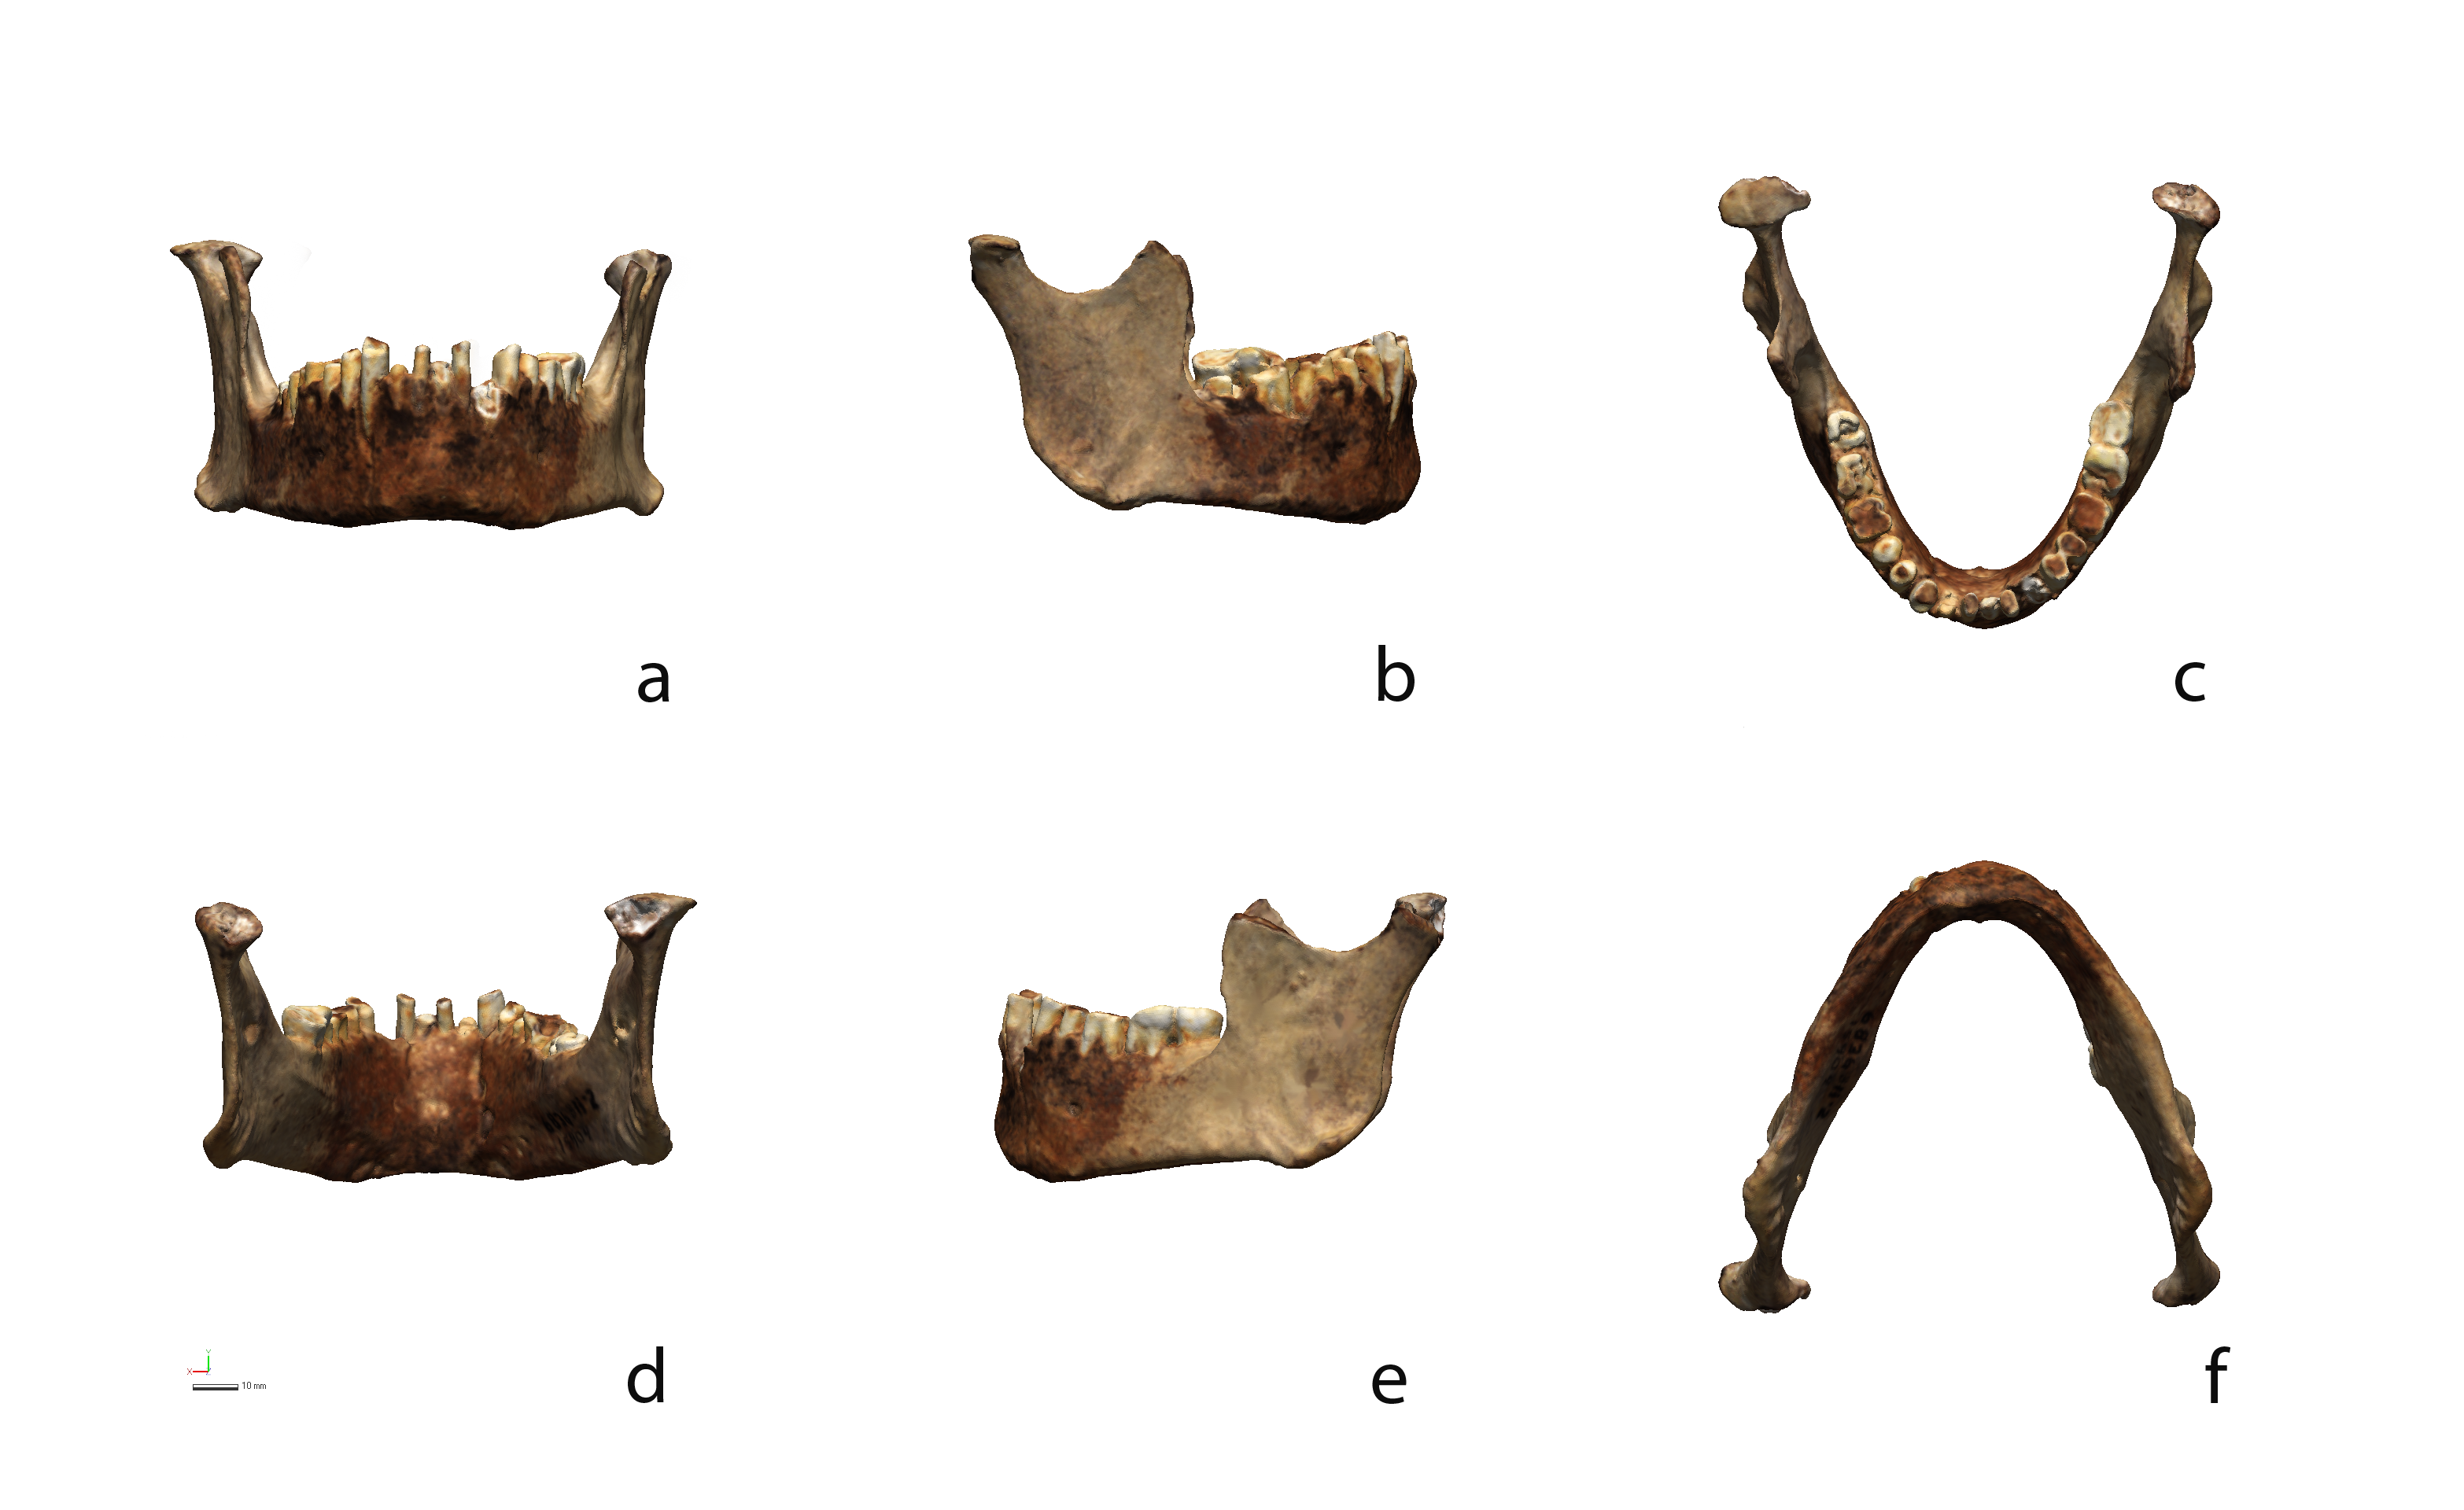
\includegraphics[width=\linewidth]{Fig1}
\caption{Surface scan data (with texture) for Mesolithic mandible B11-2-15904 from the Kulubnarti collection; illustrating (a) anterior, (b) right buccal, (c) superior, (d) posterior, (e) left buccal, and (f) inferior views.}
\label{fig:Fig2}
\end{figure}

Following data collection, the mandible was modeled in Dx using a custom patch network designed to capture the high detail of the mesh in a surface model. Three-dimensional contour curves were applied along high curvature areas of the mesh that were used as the basis for the initial layout of the custom patch network. The first iteration of the custom patch network enlisted an auto estimation for the number of patches necessary, which was subsequently refined through a series of iterative comparisons between the surface model and the mesh by moving between Dx and Geomagic Control X (Cx).

Throughout the design and layout process for the custom patch network, each iteration of the freeform surface model was exported to Cx to identify areas of the surface model’s design that exceeded the specified---arbitrary---tolerance ( 0.1 mm; same as post-processed mesh resolution) and required revision. Development of the final surface model was an iterative process resulting in a total of three revisions, yielding a freeform surface model where 100 percent of the surface model is within the  0.1 mm tolerance of the mesh. Revisions to the custom patch network were conducted by shuffling patch groups, editing, and inserting splines. The final freeform surface model was then exported to Cx for comparisons with the processed CT-rendered model. While surface scan data are used as the control, this is not meant to convey a measure of accuracy; rather, these data are used to identify the CT post-processing method that yields the mesh with the smallest deviation between the surface model and CT-generated data.

\subsection*{Computer-Aided Inspection}

Cx was used to compare the topology of the surface model (nominal data) against that of the eight CT meshes (measured data) \citep{RN11473} (Figure ~\ref{fig:Fig1x}). Measured data was compared against the nominal data \citep{RN11463,RN5923,RN11460,RN11465} to identify the method of CT post-processing that best fits with the surface model based upon the percentage of the 3-D mesh that meets with a pre-specified---arbitrary---tolerance (0.3 mm) \citep{RN5925,RN11471,RN11455}. Once identified, a series of two-dimensional (2D) slices were generated for the CT mesh that best fit with the surface scan to further clarify the character of the geometric shapes associated with gap distances.

\begin{figure}[ht]\centering
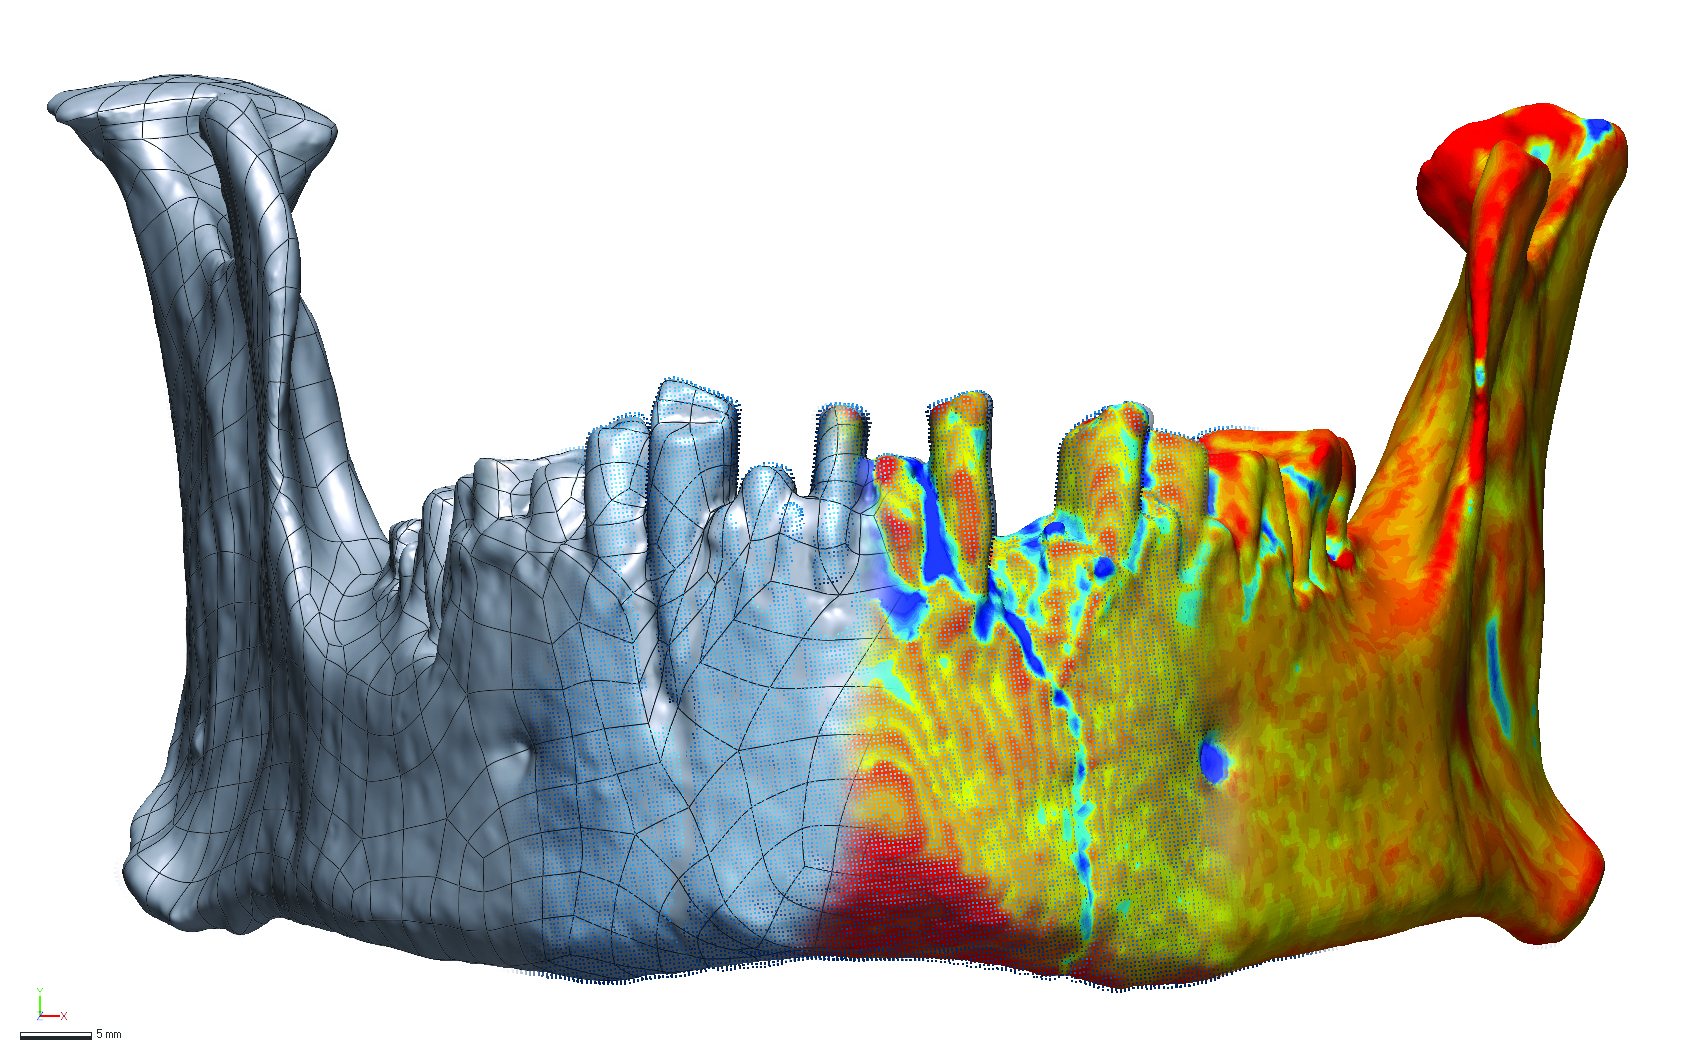
\includegraphics[width=\linewidth]{Fig2}
\caption{Surface model (left) contrasted with CT point cloud (centre) and gap distances between the surface model and CT mesh (right). \textit{Inspection tolerance was altered to 0.05 mm to more dramatically illustrate deviations that occur between the mesh and surface model for this figure}.}
\label{fig:Fig1x}
\end{figure}

A total of thirty-three \textit{reference points} were populated on the mesh in Dx (Figure ~\ref{fig:Fig4}). These points were placed in the vicinity of mandibular landmarks (e.g., menton), which were specifically chosen due to their use in an unrelated study of the Mesolithic Kulubnarti mandibles \citep{RN11477}. These \textit{reference points} were saved as an initial graphics exchange specifications (IGES) file, and they were then imported to Cx as \textit{comparison points}, with the purpose of using the \textit{comparison points} to assess deviations among the various models at known locations of analytical importance. Note that \textit{comparison points} associated with the fractured left condyle of the mandible were not reflected here as they were in the geometric morphometric study \citep{RN11477}. A number of methods have been proposed to reconstruct \citep{RN11496,RN11501} or otherwise account for missing data in geometric morphometrics \citep{RN11500,RN11497,RN11498,RN11499,RN5928}, none of which were used here. Instead, \textit{comparison points} were placed atop the area of the fracture, which afforded an opportunity to explore how a region of highly variable geometry would compare between the surface model and the CT meshes.

\begin{figure}[ht]\centering
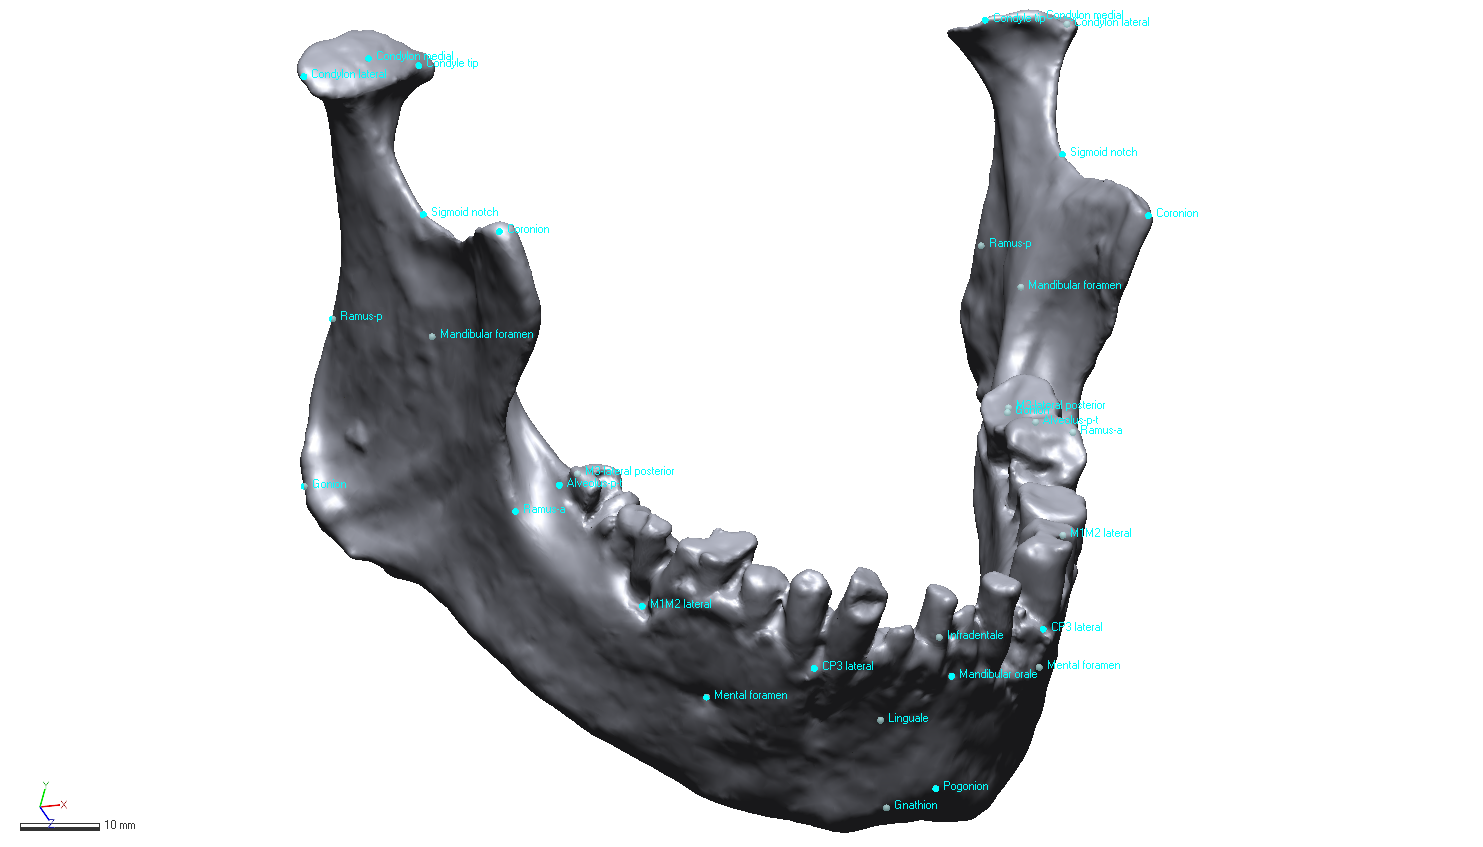
\includegraphics[width=\linewidth]{Fig4}
\caption{Location of the 33 landmarks used in \citet[Supplementary Information]{RN11477} which were populated on the surface model in Dx, and imported as \textit{comparison points} to Cx.}
\label{fig:Fig4}
\end{figure}

\section*{Results}

Comparisons are limited to the topology of the surface model due to the fact that it is not possible to capture interior structures with a surface scanner. It is, however, possible to compare the topology of the CT mesh against that of the surface scan by limiting the analysis to the topology of the faces of the surface model. 

\subsection*{Mesh comparison (3-D compare)}

The 3-D comparisons of the surface model with the eight CT meshes suggest that the M1 \textit{HMH 0 smooth} mesh (inTol 93.92\%) and the M2 \textit{HMH 0} mesh (inTol 93.80\%) correlate best with the surface model when the entirety of the mandible geometry---100\% sampling ratio---is compared (Figure ~\ref{fig:Fig3}, Table ~\ref{tab:Tbl2}). CT meshes M3 and M4 \textit{HMH -500 smooth} and \textit{HMH -500}, demonstrate the lowest tolerance levels (InTol 62.20\% for both), thus correspond least to the surface scan. Additional comparisons indicate that high gap distances occur primarily in regions between dentition and around the mental foramina. Deviations also occur on the anterior rami and condyles, particularly in the area of the fractured left condylar neck. 

\begin{figure}[ht]\centering
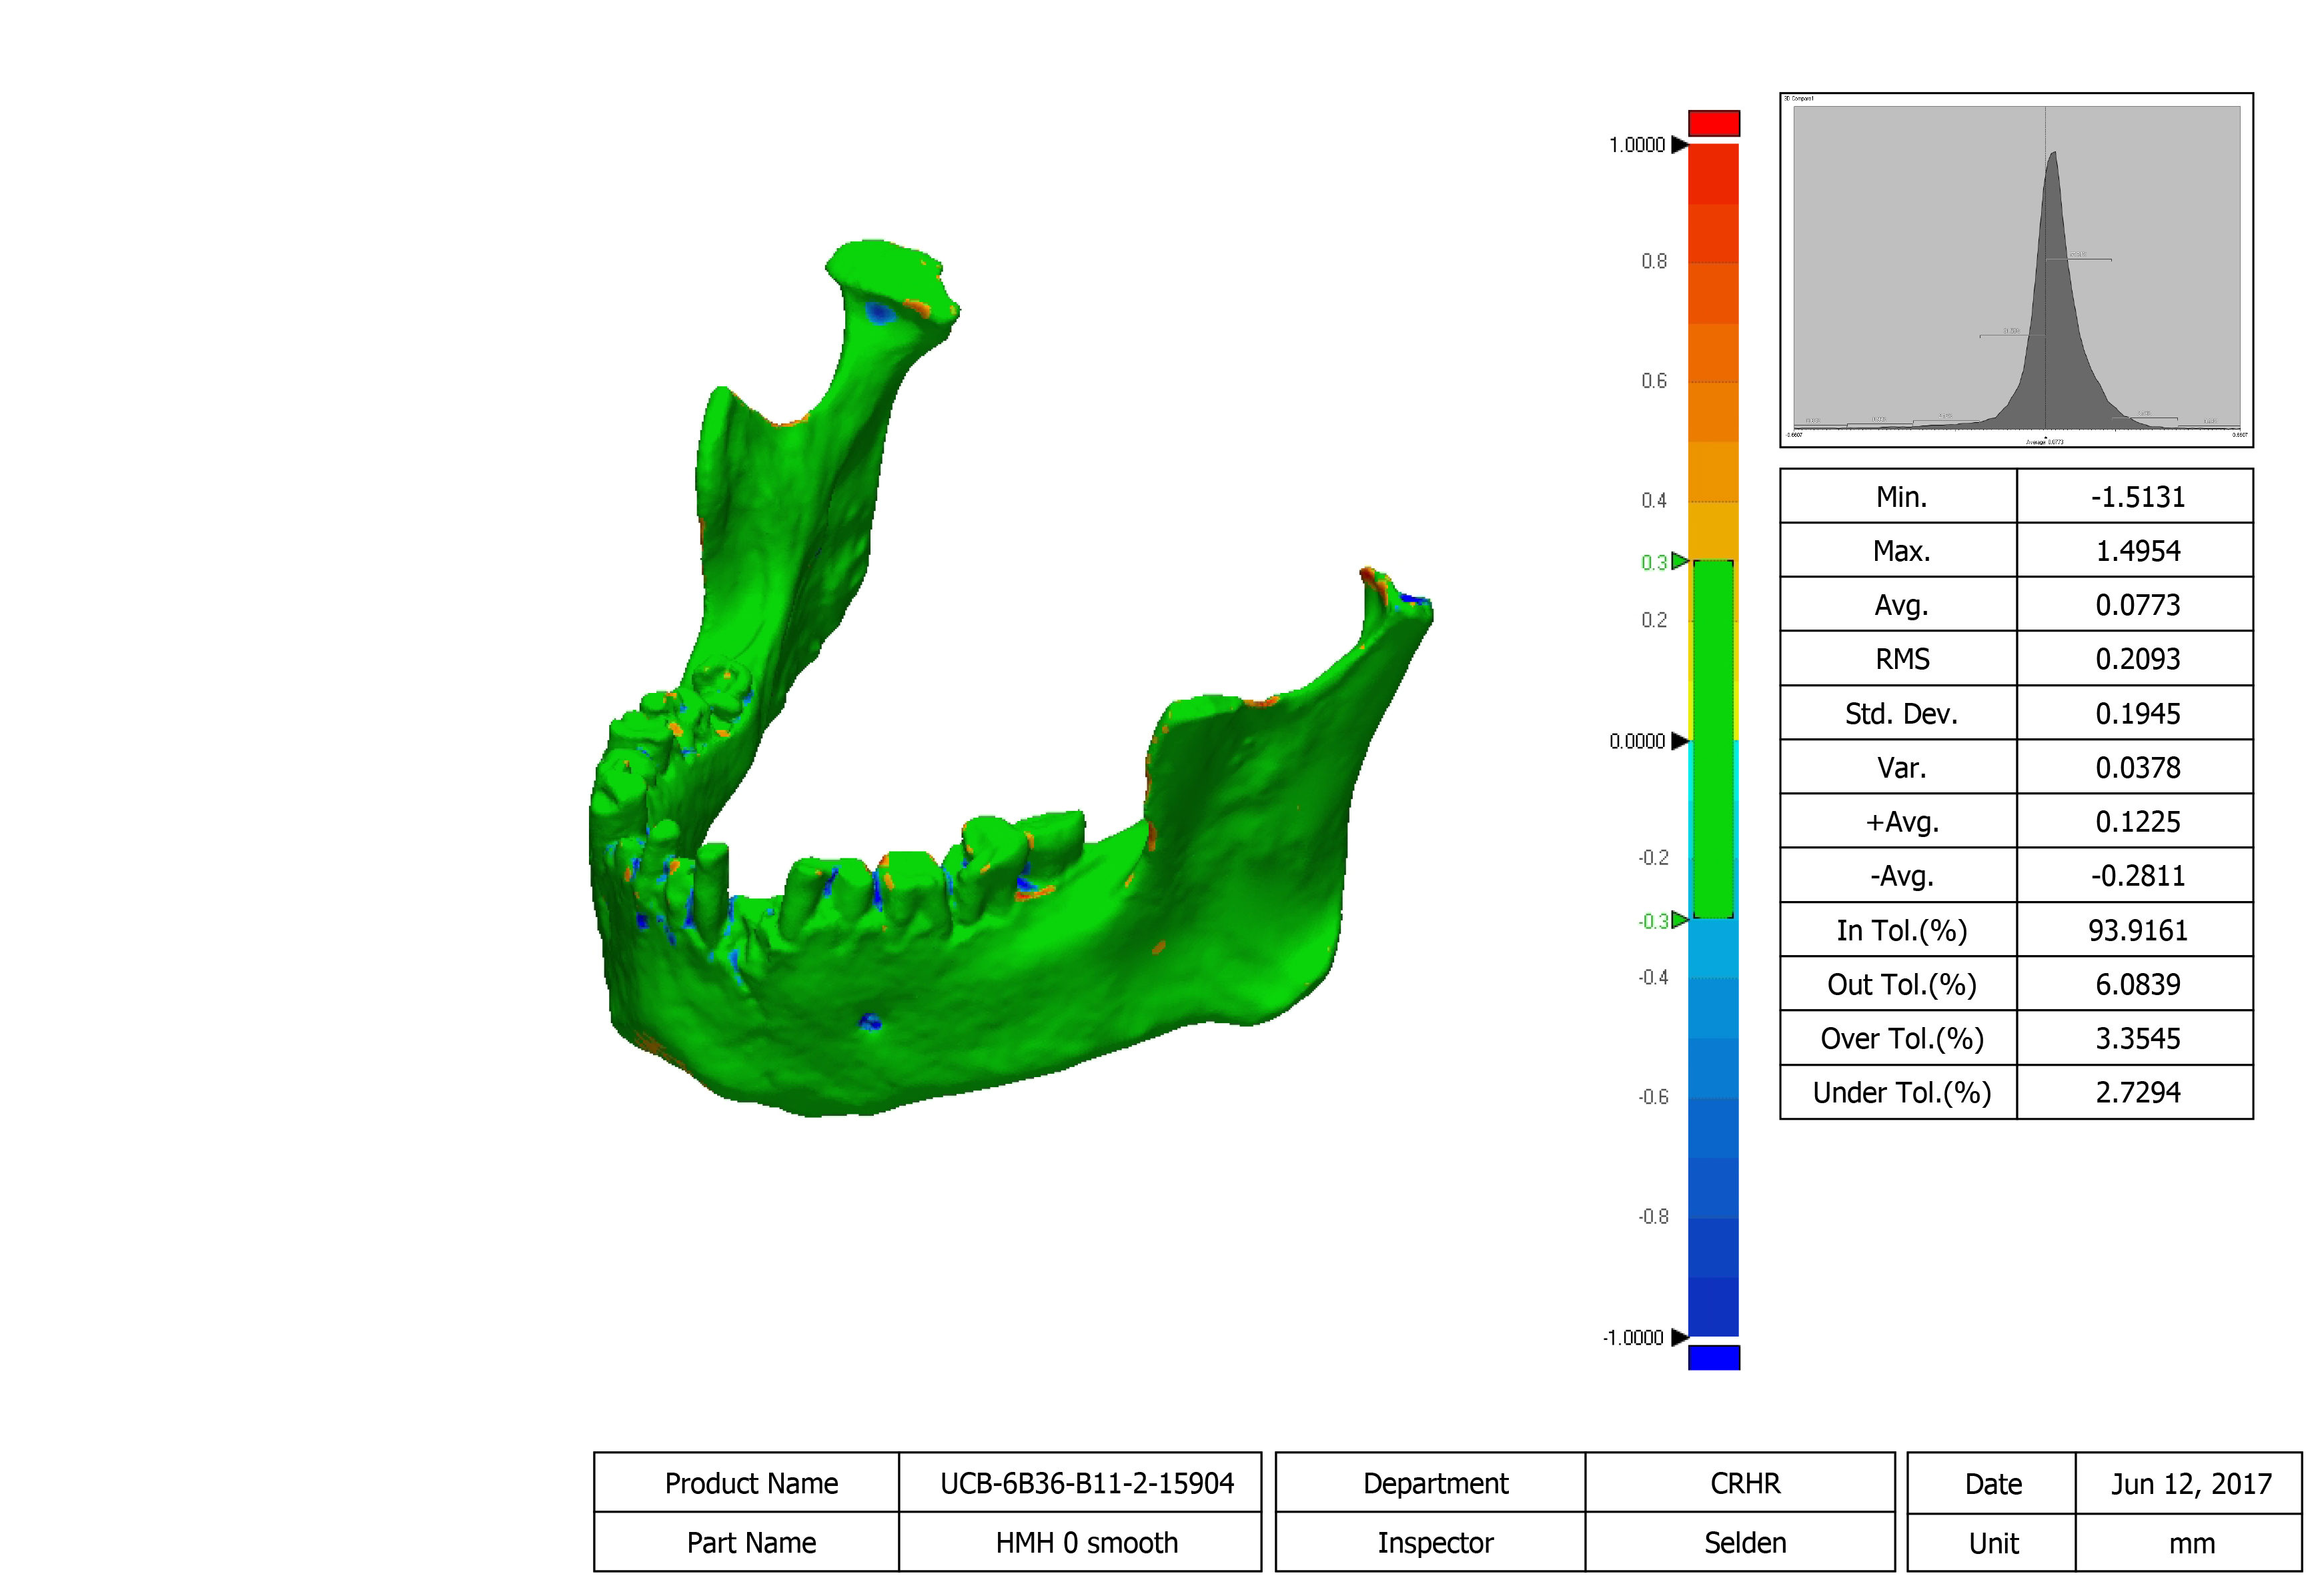
\includegraphics[width=\linewidth]{Fig3}
\caption{Comparison between the surface model and the thresholding methods (isosurfacing) for \textit{HMH 0 smooth}; regions of mesh topology in green represent the geometry of Mesolithic mandible B11-2-15904 in the $\pm$ 0.3 mm tolerance.}
\label{fig:Fig3}
\end{figure}

The histogram shown in Figure ~\ref{fig:Fig3} illustrates the Gaussian distribution for the number of errors over the whole deviation. The graph is split into six segments: 1-Sigma at 31 percent from the average to the maximum deviation in each direction, 2-Sigma at 69 percent from the average to the maximum deviation in each direction, and 3-Sigma at 93.3 percent from the average to the maximum deviation in each direction. The average (AVG) is the sum of all deviations divided by the number of all deviations, and the RMS is the square root of all squared deviations divided by the number of all deviations (sometimes referred to as the effective deviation). In tolerance (In Tol) and out tolerance (Out Tol) percentages indicate the percentage of deviations in or out of the given tolerance, and over tolerance (Over Tol) and under tolerance (Under Tol) percentages indicate the percentage of deviations over (positive direction) or under (negative direction) the tolerance range. 

\begin{table}[tbh]\centering
\footnotesize
\caption{Results of 3-D comparison between surface scan and CT meshes}
\centering
\begin{tabular}{lcccc}
\hline
CT Mesh & InTol (\%) & OutTol (\%) & OverTol (\%) & UnderTol (\%)\\
\hline
M1 & 93.9161 & 6.0839 & 3.3545 & 2.7294\\
M2 & 93.8012 & 6.1988 & 3.4278 & 2.771\\
M3 & 62.1989 & 37.8011 & 2.0537 & 35.7474\\
M4 & 62.2013 & 37.7987 & 2.0499 & 35.7488\\
M5 & 90.5318 & 9.4682 & 8.6902 & 0.7779\\
M6 & 88.3977 & 11.6023 & 10.8934 & 0.709\\
M7 & 87.4393 & 12.5607 & 11.9468 & 0.6139\\
M8 & 87.4647 & 12.5353 & 11.8925 & 0.6428\\
\hline
\end{tabular}
\label{tab:Tbl2}
\end{table}

\subsection*{2D sectioning (2D compare)}

The 2D comparison was generated for four sections of \textit{HMH 0 smooth} at, or very near locations on the mesh where comparison points were later applied (Table ~\ref{tab:Tbl3} and Figure ~\ref{fig:Fig4}). For each of the 2D compare sections, two call-outs were added to illustrate the maximum measures of over/under tolerance. The single exception to the call-out protocol is 2D compare 3, as those gap distances associated with the mental foramina were of particular interest. In the case of 2D compare 3, the two call-outs were issued for the two highest deviations that occur under the $\pm$ 0.3 mm tolerance. 

\begin{table}[tbh]\centering
\footnotesize
\caption{Results of sectioning (2D compare) for \textit{HMH 0 smooth} in high-deviation regions of the surface scan/CT mesh near the locations of landmark data.}
\centering
\begin{tabular}{lcccc}
\hline
2D compare & InTol (\%) & OutTol (\%) & OverTol (\%) & UnderTol (\%)\\
\hline
2D compare 1 & 56.2259 & 43.7741 & 41.7202 & 2.0539\\
2D compare 2 & 88.5312 & 11.4688 & 4.829 & 6.6398\\
2D compare 3 & 93.9781 & 6.0219 & 0.6691 & 5.3528\\
2D compare 4 & 80.0948 & 19.9052 & 14.218 & 5.6872\\
\hline
\end{tabular}
\label{tab:Tbl3}
\end{table}

Through sectioning the specific CT mesh found to best fit the surface scan, variation between the surface scan and the \textit{HMH 0 smooth} mesh is better illustrated (Figure ~\ref{fig:Fig6}). Even in the most ideal cases, some areas of the mesh may not be well-suited for semilandmarks. For example, it would take substantial effort to identify areas of the left fractured condylar neck, left anterior ramus, left mandibular foramen, and both mental foramina where landmarks and semilandmarks would be deemed acceptable for inclusion in a formal analysis. However, a number of other areas remain on the \textit{HMH 0 smooth} mesh that are likely suitable for use in a mixed-method analysis, but would depend on the specifics of the research question.

\begin{figure}[ht]\centering
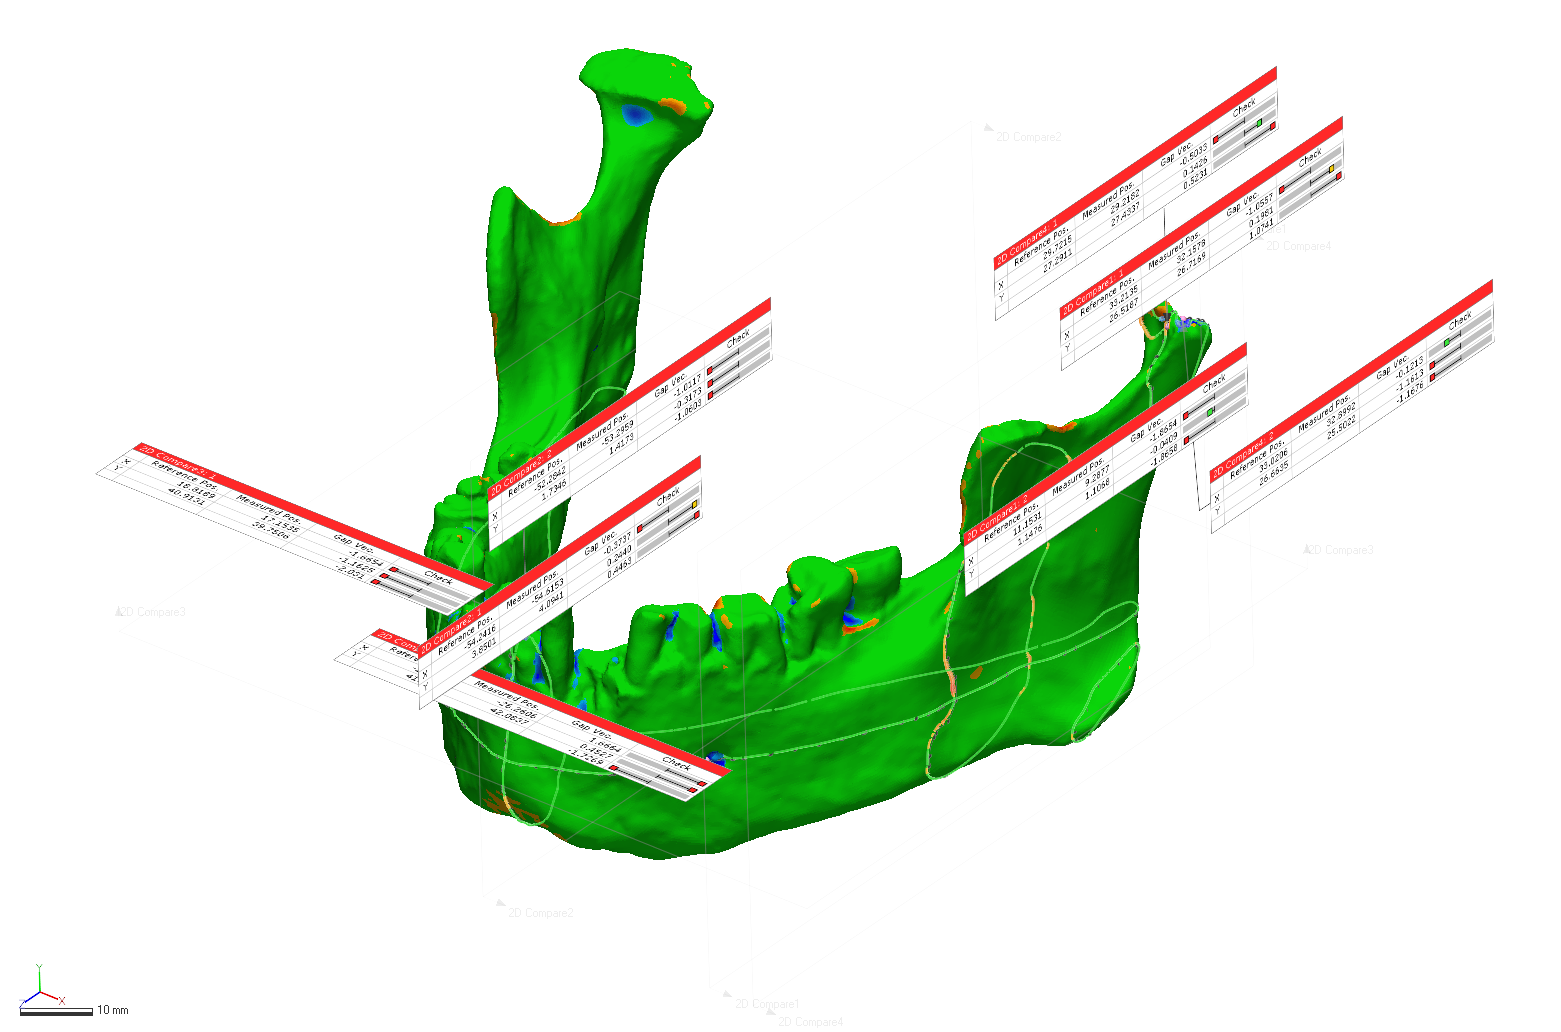
\includegraphics[width=\linewidth]{Fig6}
\caption{Surface scan contrasted with CT mesh \textit{HMH 0 smooth}, illustrating four 2D compare sections that occur at or near the location of landmarks used in an unrelated study.}
\label{fig:Fig6}
\end{figure}

\subsection*{Comparison points}
Figure~\ref{fig:Fig4} illustrates the placement of comparison points, and Figure~\ref{fig:Fig5} demonstrates the gap distance for comparison points between the surface model (reference position) and each of the eight meshes (measured position) in Cx. Gap distances were recorded (Table ~\ref{tab:Tbl4} and Supplementary Information), and results are listed in order for the eight post-processing methods. Comparison points placed on the gnathion, gonion, and pogonion showed low (in-tolerance) gap distances, while other anatomical regions demonstrated gap distances that were above tolerance for at least one of the CT meshes.

\begin{figure}[ht]\centering
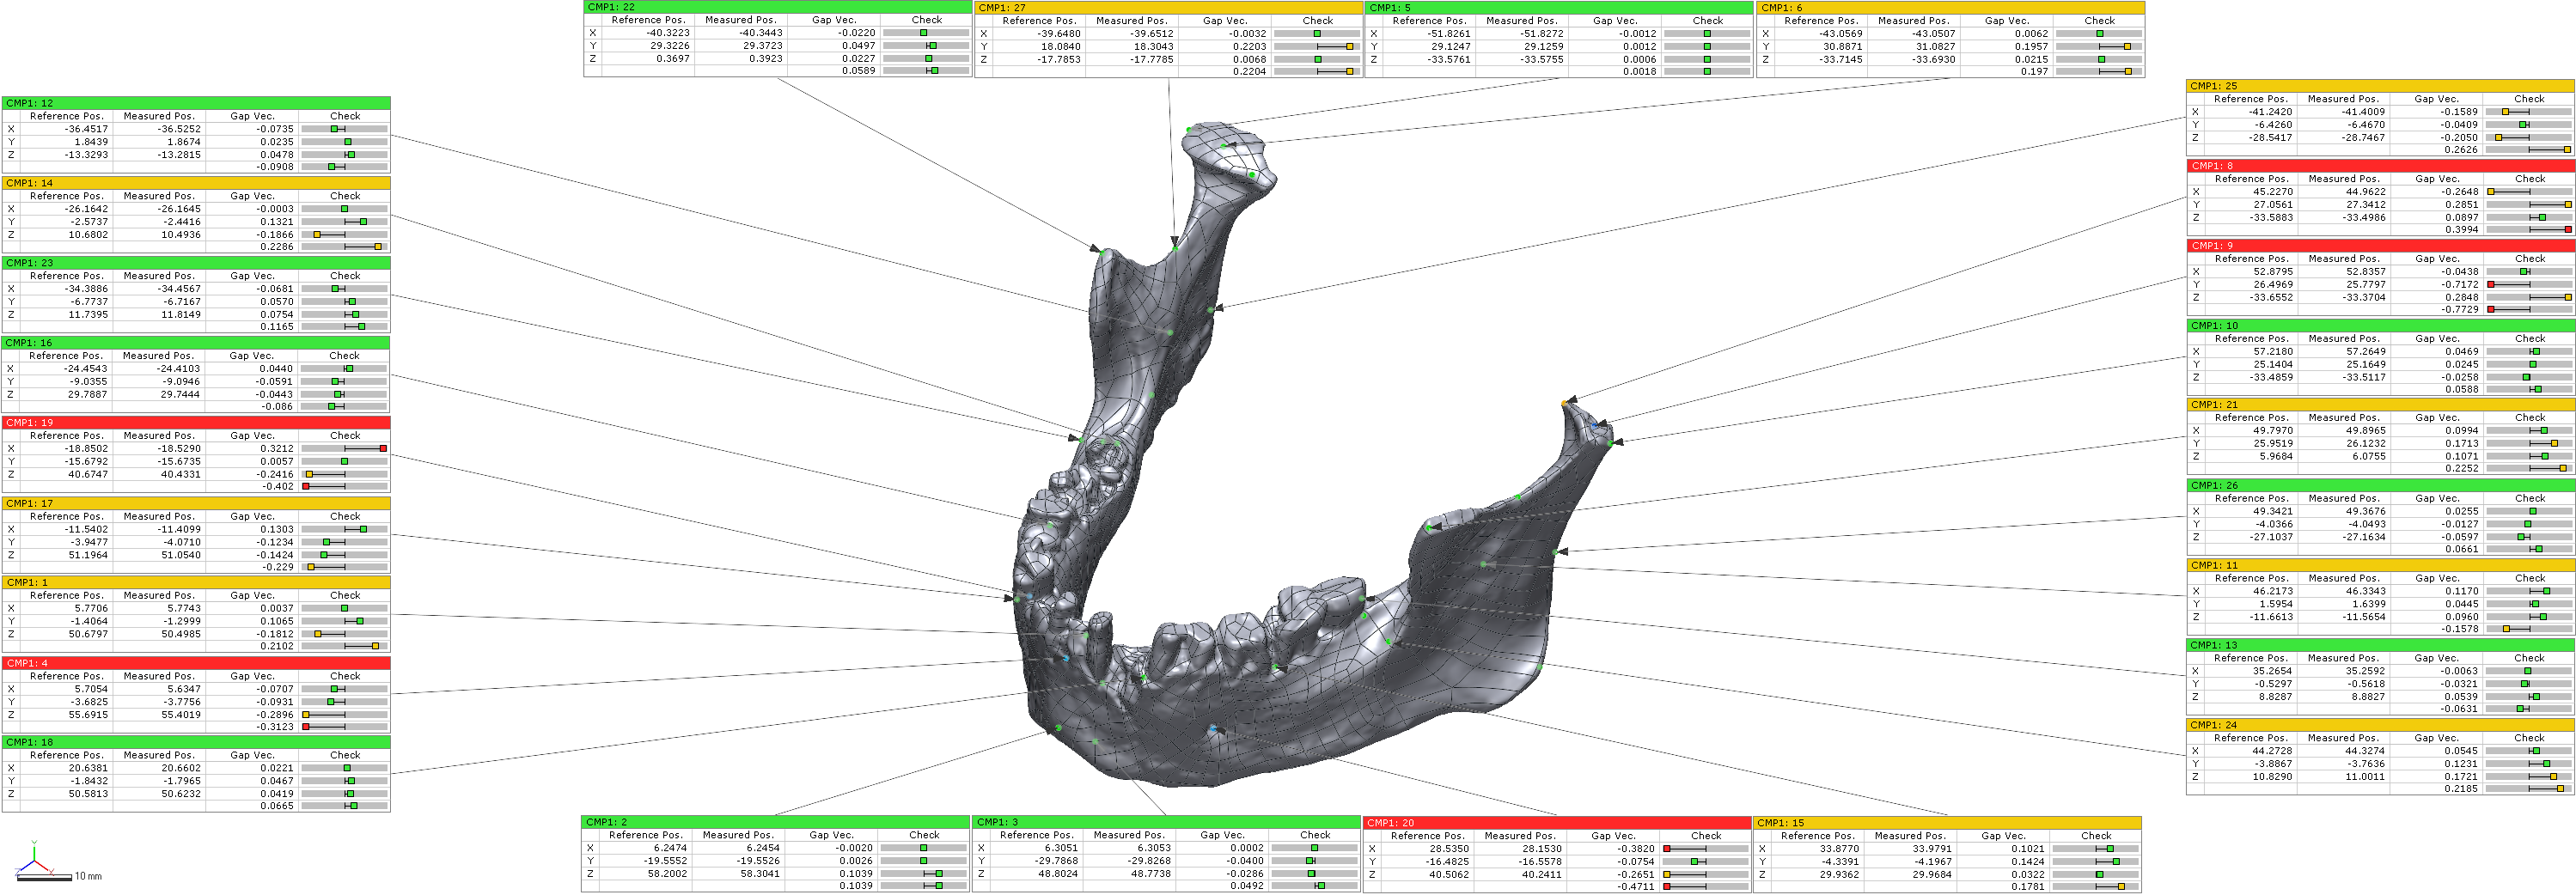
\includegraphics[width=\linewidth]{Fig5}
\caption{Surface model and comparison points contrasted with CT mesh \textit{HMH 0 smooth}, illustrating the locations for measured positions and gap vectors associated with locations used in an unrelated geometric morphometric analysis \cite[Supplementary Information]{RN11477}. Green boxes denote a comparison point within tolerance; yellow boxes indicate a comparison point within tolerance, but above/below $\pm$ 0.15 mm; and red boxes indicate a comparison point beyond the $\pm$ 0.3 mm tolerance. \textit{Importantly, these are not landmark-to-landmark measures; rather, they reflect the gap distance between the surface model and CT mesh at the location of the comparison point on the surface model}.}
\label{fig:Fig5}
\end{figure}

\begin{center}
\footnotesize
\begin{longtable}{lrrrrrrrr}
\caption{Gap distances between points at landmarks applied to the surface scan contrast with the post-processed CT meshes (see also Supplementary Data). Gap distances for points above the $\pm$ 0.3 mm tolerance are indicated in italics, and those above the $\pm$ 0.15 median are indicated in bold.} 
\label{tab:Tbl4}\\

\hline 
\multicolumn{1}{l}{CMP1} & \multicolumn{1}{r}{M1} & \multicolumn{1}{r}{M2} & \multicolumn{1}{r}{M3} & \multicolumn{1}{r}{M4} & \multicolumn{1}{r}{M5} & \multicolumn{1}{r}{M6} & \multicolumn{1}{r}{M7} & \multicolumn{1}{r}{M8}\\ 
\hline 
\endfirsthead

\multicolumn{9}{c}%
{\tablename \thetable{} -- continued from previous page} \\
\hline 
\multicolumn{1}{l}{CMP1} & \multicolumn{1}{r}{M1} & \multicolumn{1}{r}{M2} & \multicolumn{1}{r}{M3} & \multicolumn{1}{r}{M4} & \multicolumn{1}{r}{M5} & \multicolumn{1}{r}{M6} & \multicolumn{1}{r}{M7} & \multicolumn{1}{r}{M8}\\  
\hline 
\endhead

\hline 
\multicolumn{9}{r}{{Continued on next page.}}\\
\hline
\endfoot

\endlastfoot

CMP1:1 & \textit{0.2102} &\textit{0.198}& \textbf{0.8376} & \textbf{0.8376} & 0.0177 & 0.004 & -0.0327 & -0.038\\
CMP1:2 & 0.1039 & 0.1039 & 0.1391 & 0.1391 & -0.0285 & -0.0284 & -0.0444 & -0.044 \\
CMP1:3 & 0.0492 & 0.04 & 0.0282 & 0.0282 & -0.0968 & -0.1175 & -0.1226 & -0.1388 \\
CMP1:4 & \textbf{-0.3123} & \textit{-0.2804} & \textit{-0.1671} & \textit{-0.1671} & \textbf{-0.8656} & \textbf{-1.4265} & \textbf{-0.8968} & \textbf{-0.886}\\
CMP1:5 & 0.0018 & -0.0155 & \textit{0.2077} & \textit{0.2077} & \textit{-0.2104} & \textit{-0.2174} & \textbf{-0.3048} & \textit{-0.2231}\\
CMP1:6 & \textit{0.197} & \textit{0.1987} & \textbf{0.8456} & \textbf{0.8456} & 0.0359 & 0.0212 & 0.0175 & 0.0028 \\
CMP1:7 & \textit{0.2646} & \textit{0.2548} & \textbf{0.7939} & \textbf{0.7939} & 0.1371 & 0.1328 & 0.1113 & 0.1114 \\
CMP1:8 & \textbf{0.3994} & \textbf{0.4374} & \textbf{0.6508} & \textbf{0.6508} & \textit{0.2929} & \textbf{0.3474} & \textbf{-1.3983} & \textit{0.2749}\\
CMP1:9 & \textbf{-0.7729} & \textbf{-0.8551} & \textbf{0.5884} & \textbf{0.5884} & \textbf{-1.3955} & \textbf{-1.32} & \textbf{0.2443} & \textbf{-1.4029}\\
CMP1:10 & 0.0588 &  0.0669 & \textbf{0.453} & \textbf{0.453} & -0.0948 & -0.066 & -0.1211 & -0.1137\\
CMP1:11 & \textit{-0.1578} & \textit{-0.1501} & -0.031 & -0.031 & \textbf{-0.4135} & -0.1154 & \textbf{-0.4518} & \textbf{-0.5055}\\
CMP1:12 & -0.0908 & \textit{-0.1584} & \textbf{-0.3432} & \textbf{-0.3432} & \textit{-0.2536} & \textit{-0.2413} & \textit{-0.2675} & \textit{-0.2661}\\
CMP1:13 & -0.0631 & -0.0789 & \textbf{0.5405} & \textbf{0.5405} & \textit{-0.2241} & \textit{-0.2489} & \textit{-0.2452} & \textit{-0.2716}\\
CMP1:14 & \textit{0.2286} & \textit{0.1974} & \textbf{1.0348} & \textbf{1.0348} & 0.0213 & 0.0157 & 0.0038 & -0.0056\\
CMP1:15 & \textit{0.1781} & \textit{0.164} & \textbf{0.6065} & \textbf{0.6065} & -0.0065 & -0.027 & -0.0217 & -0.0462\\
CMP1:16 & -0.086 & -0.0628 & \textbf{0.3406} & \textbf{0.3406} & \textbf{-0.4628} & \textbf{-0.3485} & \textbf{-0.3469} &\ \textbf{-0.3778}\\
CMP1:17 & \textit{-0.229} & \textit{-0.202} & 0.0696 & 0.0696 & \textbf{-0.5577} & \textbf{-0.5415} & \textbf{-0.6697} & \textbf{-0.6833}\\
CMP1:18 & 0.0665 & 0.0914 & \textbf{0.5026} & \textbf{0.5026} & -0.1306 & -0.1262 & \textit{-0.1501} & -0.1468\\
CMP1:19 & \textbf{-0.402} & \textit{-0.1847} & \textbf{-0.9968} & \textbf{-0.9968} & \textbf{-0.6075} & \textbf{-0.7322} & \textbf{-0.6367} & \textbf{-0.7859} \\
CMP1:20 & \textbf{-0.4711} & \textbf{-0.4646} & \textbf{-0.9352} & \textbf{-0.9352} & NR & NR & NR & NR\\
CMP1:21 & \textit{0.2252} & \textit{0.2366} & \textbf{0.5418} & \textbf{0.5418} & 0.1066 & 0.1085 & 0.0866 & 0.0928\\
CMP1:22 & 0.0589 & 0.048 & \textbf{0.3684} & \textbf{0.3684} & -0.042 & -0.0662 & -0.0697 & -0.0803\\
CMP1:23 & 0.1165 & 0.1147 & \textit{0.2853} & \textit{0.2853} & 0.0068 & -0.0009 & -0.0046 & -0.0143\\
CMP1:24 & \textit{0.2185} & \textit{0.217} & \textbf{0.3651} & \textbf{0.3651} & 0.0906 & 0.0913 & 0.0817 & 0.077\\
CMP1:25 & \textit{0.2626} & \textit{0.2531} & \textbf{0.5859} & \textbf{0.5859} & 0.1163 & 0.0895 & 0.094 & 0.0698\\
CMP1:26 & 0.0661 & 0.0647 & \textbf{0.3943} & \textbf{0.3943} & -0.0533 & -0.0649 & -0.0693 & -0.0809\\
CMP1:27 & \textit{0.2204} & \textit{0.2262} & \textbf{0.8613} & \textbf{0.8613} & 0.1201 & 0.0958 & 0.0963 & 0.0711\\
CMP1:28 & \textit{0.2085} & \textit{0.2244} & \textbf{0.6433} & \textbf{0.6433} & 0.0578 & 0.0949 & 0.0358 & 0.0771\\
CMP1:29 & \textit{0.2191} & \textit{0.2313} & \textbf{0.8063} & \textbf{0.8063} & 0.0186 & 0.0282 & 0.0105 & 0.0027\\
CMP1:30 & 0.1127 & 0.1035 & \textbf{0.471} & \textbf{0.471} & -0.0393 & -0.0656 & -0.0519 & -0.084\\
CMP1:31 & 0.1294 & 0.1415 & \textbf{0.4371} & \textbf{0.4371} & -0.0196 & 0.0042 & -0.0307 & -0.0141\\
CMP1:32 & 0.135 & 0.1288 & 0.0266 & 0.0266 & 0.0317 & 0.025 & 0.0077 & 0.0125\\
CMP1:33 & 0.0549 & 0.0474 & 0.1231 & 0.1231 & -0.0414 & -0.0476 & -0.0555 & -0.058\\
\hline\\
\caption*{\textit{CMP1 = comparison point; M1 = HMH 0 smooth; M2 = HMH 0; M3 = HMH -500 smooth; M4 = HMH -500; M5 = HMH 562 smooth; M6 = HMH 562; M7 = HMH 634 smooth; M8 = HMH 634;NR = No Result; CMP1:1 = Infradentale; CMP1:2 = Pogonion; CMP1:3 = Gnathion; CMP1:4 = Mandibular orale; CMP1:5 = Condylon lateral (R); CMP1:6 = Condylon medial (R); CMP1:7 = Condylon tip (R); CMP1:8 = Condylon tip (L); CMP1:9 = Condylon medial (L); CMP1:10 = Condylon lateral (L); CMP1:11 = Mandibular foramen (L); CMP1:12 = Mandibular foramen (R); CMP1:13 = M3-lateral posterior (L); CMP1:14 = M3-lateral posterior (R); CMP1:15 = M1M2 lateral (L); CMP1:16 = M1M2 lateral (R); CMP1:17 = CP3 lateral (R); CMP1:18 = CP3 lateral (L); CMP1:19 = Mental foramen (R); CMP:20 = Mental foramen (L); CMP:21 = Coronion (L); CMP:22 = Coronion (R); CMP:23 = Ramus-a (R); CMP:24 = Ramus-a (L); CMP:25 = Ramus-p (R); CMP:26 = Ramus-p (L); CMP:27 = Sigmoid notch (R); CMP:28 = Sigmoid notch (L); CMP:29 = Linguale; CMP:30 = Alveolus-p (L); CMP:31 = Alveolus-p (R); CMP:32 = Gonion (R); CMP:33 = Gonion (L).}}
\end{longtable}
\end{center}

Comparison points placed around landmarks across the different CT meshes did not correspond well, with several exhibiting gap distances above the $\pm$ 0.3 mm tolerance. The CT meshes that best correspond with the repurposed constellation of comparison points were M1 and M2 (\textit{HMH 0 smooth} and \textit{HMH 0}). For these meshes, only three comparison points extend beyond the $\pm$ 0.3 mm tolerance: condylon tip (L), condylon medial (L), and mental foramen (L). It is important to reiterate, however, that the two measures atop the left condyle were collected in the area of a fracture, so this result is not unexpected (see discussion, below). The meshes displaying the highest gap distances were the M3 and M4 CT-meshes (\textit{HMH -500 smooth} and \textit{HMH -500}). It is worth noting that while mesh topology for M3 and M4 does vary in terms of the 3-D compare analyses, gap distances for comparison points were exactly the same. Results for the M5 - M8 meshes are also similar in terms of which landmarks extended beyond the median and maximum tolerance. In total, four landmarks remain below the median tolerance for \textit{all} meshes (pogonion, gnathion, gonion [R], and gonion [L]), and only one landmark included a gap distance reaching only the median tolerance (ramus-a [R]). For the remainder of the comparison points, at least one extended beyond the maximum tolerance for all CT models (Table ~\ref{tab:Tbl4}). 

\section*{Discussion}

Eight CT meshes were digitally rendered using different thresholding parameters, then compared to a single 3-D surface model to identify the post-processing method for CT scans that produces the smallest gap distances in terms of surface topology (3-D comparisons), the sections most suitable for landmark and/or semilandmark placement (2D section comparisons), and the smallest gap distances in terms of landmark placement (comparison point analyses). All three analyses demonstrate that post-processing methods impact the comparability of the 3-D meshes that are the primary data source used in studies of 3-D geometric morphometrics. Thus, if conducting a mixed-method study, incorporating those analyses employed here would be beneficial to identify which post-processing techniques yield the most consistent mixed-method dataset needed to addresses a specific research question, while also highlighting those aspects of mesh geometry most suitable for landmark and semilandmark application in more advanced studies. As detailed below, it is recommended that unprocessed data be made available in addition to processed 3-D meshes, making it possible to achieve consistent data processing for studies where reuse is possible, as well as replication studies where the processed mesh can be used.

\subsection*{Mesh comparison (3-D Compare)}

Results indicate that the neutral CT-mesh M1, \textit{HMH 0 smooth}, is the best match to the surface model in terms of overall model composition; however, this result does not necessarily mean that the \textit{HMH 0 smooth} mesh is the most biologically accurate. As mentioned previously, numerous studies  \citep{RN11483,RN11485,RN11486} have demonstrated that post-processing techniques, which include the HMH-technique for objectively determining appropriate thresholding values depending on the material involved, are extremely important for obtaining accurate models and measurements. Despite this, studies enlisting CT meshes continue to use subjective methods and/or do not provide additional processing information.

It is likely that the appropriate post-processing methods for one study will not translate across multiple studies, as research interests tend to be wide-ranging. With this in mind, it is recommended that researchers pay particular attention when selecting the appropriate processing method. If mixed-method data cannot be avoided, preliminary comparative analyses that contrast results of differential post-processing techniques may be warranted. When obtaining CT, laser, structured light, etc. from websites and digital repositories, it is important that post-processing methods---or stages---be thoroughly identified, understood, and communicated; and these data should be provided with each (see \cite{RN11502} for a recent review of MorphoSource, and \cite{RN11503} for a recent review of MorphoMuseum). In cases of 3-D data, it best to use the original files where possible (e.g., .tiff stacks, analyse files, Dicoms, etc.), versus simply posting processed models/meshes. This would ensure that models and meshes can be rendered in a manner that yields consistent outputs for a specific project \citep{RN8984}. For example, a project that is focused upon dentition may use different thresholding techniques compared to that of a project focused on mandibular bone, femur, pelvis, etc.

\subsection*{2D sectioning (2D compare)}

Although an important first step, the complex variability for two or more specimens identified through the first comparison (3-D compare) requires two-dimensional sectioning, where gap distances can be further scrutinised, illustrated, and clarified. The contribution of the 2D compare results may be of particular importance prior to the application of semilandmarks \citep{RN4772,RN1768} and sliding semilandmarks used to analyse the morphological variability among specific, well-defined curves \citep{RN5921,RN5920}. The 2D compare sections illustrate specific areas of topology between the model and the mesh that are potentially problematic. For example, the 2D comparisons illustrates that areas of high complex morphology---here illustrated by the fractured condylar neck---may not be suitable locations for landmarks in a mixed-method dataset. Following identification of post-processing tools that result in the lowest gap distance between meshes and sections, landmark and semilandmark constellations can be refined.

\subsection*{Comparison points}

Identifying comparison points that should \textit{not} be used as positions for landmarks or semilandmarks is as important as identifying those \textit{to} use, as the mesh topology in some regions will likely be better suited for a mixed-method approach than others. Those placed in areas of complex geometry, particularly areas with deeper structures associated with dentition, mental foramina and fractures/breaks, deviate most (similar to results found in the 2D and 3-D compare analyses). This could reflect the fact that surface scanning is limited to surface topography while CT scans are capable of capturing elements of internal morphology. However, it is noteworthy that an analysis of a fully-intact mandible may result in measures for comparison points on both condyles that are within tolerance, similar to those on the intact right condyle. 

With this in mind, it is acknowledged that comparison points would not normally be placed on a broken specimen; instead, that area of the mesh would either be virtually reconstructed \citep{RN11496,RN5889,Heid1,RN5903,RN5904}, mirrored \citep{RN11504}, or otherwise treated as missing \citep{RN11500,RN11497,RN11498,RN11499}. However, the placement of landmarks on the broken neck of the left condyle in this study provides interesting insights into potential problems associated with the application of comparison points, or landmarks, for mixed-method studies of complex geometric structures. Perhaps not surprisingly, these results suggest that CT-scans may be better-suited for analyses of deeper crevices (dentition), cranial sutures, foramina, fractures, and other biological structures at the point of transition from external to internal morphology. This finding is similar to that of \citet{RN8984}, who emphasised the importance of precise processing techniques when viewing complex anatomy, including the epiphyseal plates of subadult materials.

These results represent one approach to identifying variation in mixed-methods data sets, and demonstrates the need to compare data produced using different collection and post-processing modalities prior to analysis. The comparative methodological approach can be tailored to aid in the gradual refinement of post-processing work flows when used for a single scanner coupled with omnifarious post-processing methods, algorithms, and settings used to collect, process, and model 3-D scan data \citep[22-23 and Figure 2]{RN11473}. To fully comprehend the complexities of the results, it is recommended that data are compared prior to formal analyses, allowing analysts to identify and further scrutinise specific areas of meshes that may prove problematic. Additional studies that compare modelling applications for skeletal objects (e.g., an entire cranium or post-cranial elements), cultural materials (e.g. ceramics, lithics, etc.), and proposed curve and patch elements associated with the addition and incorporation of semilandmarks or sliding semilandmarks will add important insights to the gradual identification of those processing techniques most appropriate for a wider range of mixed-method studies.

\section*{Conclusion}

Comparative studies of 3-D data processed using different suites of hardware and software are necessary to comprehend the ambiguity introduced through the use of different post-processing methods. This is of particular import when those models and/or meshes used in a study were produced for another analysis (perhaps with very different goals and data collection protocols). Scan data curated in digital archives and/or databases warrant additional scrutiny, as contextual and scan-specific metadata are neither standardised, nor required (although see \citet{RN5932,RN11507}), and too often these details are not included in the description or summary. Methods used to process 3-D data matter, and while it may be tempting to quickly download and import 3-D data collected and processed for another study, it is best to request the unprocessed data, and spend the time necessary to identify those post-processing methods best-suited to address the research question. Note that the successful identification of a post-processing work flow that achieves the smallest gap distance/deviation in one study may not represent the correct---or most appropriate---choice for another study, as variable research questions tend to focus upon different elements of mesh topology. For analyses that employ a mixed-method approach using 3-D data from digital repositories and other investigators, it is best to start by identifying the post-processing protocols that result in the most consistent whole-object variability using 3-D comparisons; followed by 2D sections to investigate potential challenges associated with a specific curve (suitable or not for semilandmarks); and suites of \textit{comparison point} constellations (suitable or not for landmarks or other point-based measures) to assess variation at a specific location prior to embarking upon the formal analysis.

\section*{Acknowledgments}

We express our gratitude to the Department of Anthropology at the University of Colorado Boulder for the requisite permissions and access needed to generate the scans of the mandibles, and to Bernard K. Means, Michael J. Shott, and Bonny Ford for their comments on an earlier draft. Our thanks go to Ramesh Karki for assistance with CT scanning at the Anschutz Medical Campus as well as Charles Musiba for facilitating various aspects of this research project. Additional thanks to Paul Sandberg and Austin Lawrence, who helped to locate samples in the Mesolithic Wadi Halfa collection.

\section*{References Cited}

\bibliography{cai}

\end{document}